\documentclass[a4paper,10.5pt]{article}
\usepackage[margin=2cm]{geometry}
\usepackage[T1]{fontenc}
\usepackage[utf8]{inputenc}
\usepackage{lmodern}
\usepackage{fontspec}
%\usefonttheme{serif}
\setmainfont{TeX Gyre Pagella}

\title{Modern IPC in Linux}
\author{Martin Sehnoutka}
\usepackage{tocloft}
\renewcommand{\cftsecleader}{\cftdotfill{\cftdotsep}}
\usepackage{xcolor}
\usepackage[pdfauthor={Martin Sehnoutka},
            pdftitle={Modern IPC in Linux},
            pdfsubject={Operating Systems},
            pdfkeywords={IPC, D-Bus, Linux},
            pdfproducer={XeTex},
            pdfcreator={pdflatex},
            colorlinks=false,
            linkbordercolor=red,% hyperlink borders will be red
            pdfborderstyle={/S/U/W 1},
	          breaklinks=true,		% Hypertextové odkazy mohou obsahovat zalomení řádku
	          hypertexnames=false]{hyperref}

\usepackage{amsmath}
\usepackage{amsfonts}
\usepackage{minted}
\usepackage{pgf-umlsd}
\usepackage{tikz-cd}
\usepackage{tikz}
\usetikzlibrary{patterns}
\usetikzlibrary{calc}
\usetikzlibrary{positioning}
\usetikzlibrary{shapes}
%\usetikzlibrary{crypto.symbols}
%\tikzset{shadows=no}        % Option: add shadows to XOR, ADD, etc.
\newcommand{\termutil}[1]{\textbf{#1}}
\newcommand{\localfile}[1]{\textit{#1}}
\newcommand{\myquote}[1]{\begin{center}\textit{"#1"}\end{center}}
\tikzstyle{arrow}= [thick, ->, >=stealth]
\tikzstyle{bsarrow}= [thick, <->, >=stealth]

\begin{document}
\begin{center}

\noindent\rule{16cm}{0.4pt}

\huge Modern IPC in Linux

\large A brief introduction to D-Bus

\noindent\rule{16cm}{0.4pt}

\end{center}

\textbf{Author:} Martin Sehnoutka

Operating System course, University of Patras

\tableofcontents

\begin{abstract}
Inter Process Communication (IPC) is an essential part of every operating system. Classic mechanisms like shared memory, unix-domain socket or pipes provide necessary IPC primitives, but their usage is complicated and way too low level for common use cases. D-Bus is a software bus abstraction, that is designed specifically for IPC in Linux desktop environment.
\end{abstract}

\section{Theoretical background}

In this section I briefly introduce theoretical background necessary for understanding D-Bus.

\subsection{What is Linux?}
Linux itself is just a kernel \footnote{Source: \url{https://www.kernel.org/category/about.html}}. It is not a small project, in fact it is probably the biggest open-source project in the world, but to create an operating system (OS), kernel itself is not enough. This is where Linux distributions are introduced. A distribution is a set of software packages, that together create a functional operating system. There is not just one distribution, in fact there are hundreds of them, because every developer or system administrator has different needs from their OS. This is the reason for introducing distributions with short life time, but newest packages (Fedora, Ubuntu) or stable, tested, but a little bit outdated packages (Debian, Red Hat Enterprise Linux) or distributions with third-party closed source components or without them etc.

A D-Bus is a package as any other component, so it is not necessarily included in every distribution, but there is a high chance, that it will be included as a part of a desktop OS.

\subsection{Classic IPC mechanisms}

Traditional IPC mechanisms are shared memory or message passing (Figure \ref{fig:ipc-classic}), where unix-domain sockets are example of message passing mechanism. These techniques are very flexible and can be used in many different ways, so they are suitable for creating more high-level abstractions on top of them.

\begin{figure}[h!]
  \begin{center}
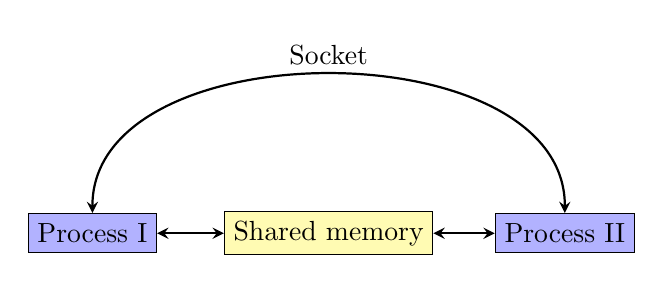
\begin{tikzpicture}[
		scale=1,
		node distance=3cm,
    rectangle/.style={
    minimum width=1cm,minimum width=1cm,minimum height=0.5cm,
    }
	]

  \node[draw,rectangle,fill=blue!30] (int) {Process I};
  \node[draw,rectangle,right of=int,fill=yellow!30] (enc) {Shared memory};
  \node[draw,rectangle,right of=enc,fill=blue!30] (int2) {Process II};
  \draw[bsarrow] (int) -- (enc);
  \draw[bsarrow] (int2) -- (enc);
  \draw (int) edge[out=90,in=90,bsarrow,out looseness=1,in looseness=1] node[above] {Socket} (int2);
\end{tikzpicture}
    \caption{Classic IPC mechanisms}
    \label{fig:ipc-classic}
  \end{center}
\end{figure}

\section{D-Bus introduction}

In this chapter, D-Bus is introduced from ideas behind it up to various implementations.

\subsection{Motivation for a new IPC mechanism}

In order to build a modern desktop operating system, many processes need to run at the same time. For instance, dhcp client, graphical desktop environment, firewall or daemon responsible for printers. In fact hundreds of processes are running at the same time. It can be counted easily using the \textbf{ps} command, which displays all running processes and then count lines using \textbf{wc}:
\begin{minted}{bash}
~ $ # Count running processes
~ $ ps -A | wc -l
310
\end{minted}

All of these processes need to communicate with each other, in order to share important information like user notifications, new hardware addition or change in network connection. There is much more possible applications for it, but they are less obvious, for those not interested in Linux desktop.

But D-Bus is not restricted to desktop environment. It can also be used for server side deployment and controlled over ssh.

\subsection{D-Bus big picture}

D-Bus, as the name suggests, is an implementation of a software bus abstraction (Figure \ref{fig:dbus}). All processes, that are connected to a bus, can see each other and communicate over the bus. The bus can be used for Remote Procedure Call (RPC) and 1-to-many publish-subscribe mechanism \footnote{Source: \url{https://www.freedesktop.org/wiki/Software/dbus/}}.

\begin{figure}[h!]
  \begin{center}
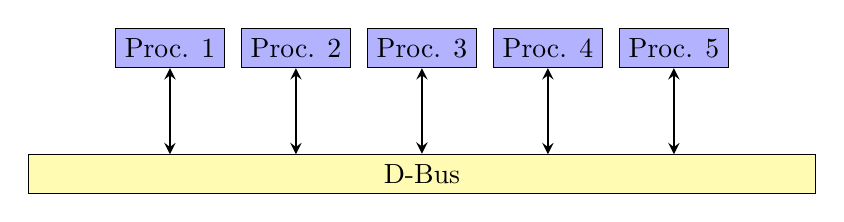
\begin{tikzpicture}[
		scale=1,
		node distance=1.6cm,
    rectangle/.style={
    minimum width=1cm,minimum height=0.5cm,
    }
	]

  \node[draw,rectangle,fill=blue!30] (p1) {Proc. 1};
  \node[draw,rectangle,right of=p1,fill=blue!30] (p2) {Proc. 2};
  \node[draw,rectangle,right of=p2,fill=blue!30] (p3) {Proc. 3};
  \node[draw,rectangle,right of=p3,fill=blue!30] (p4) {Proc. 4};
  \node[draw,rectangle,right of=p4,fill=blue!30] (p5) {Proc. 5};
  \node[draw,rectangle,below of=p3,minimum width=10cm,fill=yellow!30] (bus) {D-Bus};
  \draw[bsarrow] (p3) -- (bus);
  \draw[bsarrow] (p1) -- ++(0,-1.35);
  \draw[bsarrow] (p2) -- ++(0,-1.35);
  \draw[bsarrow] (p4) -- ++(0,-1.35);
  \draw[bsarrow] (p5) -- ++(0,-1.35);
  
  
\end{tikzpicture}
    \caption{D-Bus idea}
    \label{fig:dbus}
  \end{center}
\end{figure}

There can be multiple instances of the D-Bus running at the same time at one OS. One system-wide instance is always running, but user specific instances are created on demand, one for each login session. This comes from the obvious requirement not to mix different user sessions together. For example, one used do not want to be notified when a different one receives a new email.

\subsection{D-Bus concepts}

Terminology used in D-Bus might be little confusing at first sight. Basic building block is called a \textbf{service}, this is a running process, that is connected to a D-Bus instance and provide some \textbf{objects}. Each \textbf{service} can have multiple \textbf{objects} associated with it. For example login \textbf{service} exports one \textbf{object} for each running session.

An \textbf{object} provides one or more \textbf{interfaces}. Similarly to C\# or Java, where a programmer can define multiple interfaces for different purposes and implement them all for one class. This \textbf{interface} consist of \textbf{methods}, \textbf{signals} and \textbf{properties}. \textbf{Methods} can be used to call a remote procedure (RPC), \textbf{signals} are used to subscribe process for some notifications and \textbf{properties} define some state of a service.

Method arguments are typed using the D-Bus type system. It provides basic data types like integers or strings and basic collection types like lists and dictionaries.

Here is a list of concepts used in D-Bus \footnote{Source: \url{https://pythonhosted.org/txdbus/dbus\_overview.html}}:

\begin{itemize}
    \item \textbf{Service}(name in reverse domain notation)
    \item A program that offers some API over a bus
    \item e.g. \textit{com.example.test}
    \begin{itemize}
      \item \textbf{Object} (path notation)
      \item Each service can provide more objects, that are in tree-like hierarchy
      \item e.g. \textit{/com/example/test}
      \begin{itemize}
        \item \textbf{Interface} - a collection of \textbf{methods}, \textbf{signals} and \textbf{properties}
        \item Again in reverse domain notation
        \item e.g. \textit{com.example.test.calc}
      \end{itemize}
    \end{itemize}
  \end{itemize}
  
And overview of interface members:
\begin{itemize}
  \item Methods
  \begin{itemize}
    \item RPC mechanism
    \item Methods has a signature and a return value
    \item e.g. ss for two strings or \{is\} for dictionary\{int=>string\}
  \end{itemize}
  \item Signals
  \begin{itemize}
    \item 1-to-many publish-subscribe mechanism
    \item Client can subscribe for signals that are emitted by an object
  \end{itemize}
  \item Properties
  \begin{itemize}
    \item Like member variables in OOP
    \item with set/get methods
  \end{itemize}
\end{itemize}


\section{Command line tools and code examples}

There is not just one implementation of D-Bus specification. Different projects like GNOME, KDE or systemd has its own implementation and some programming languages like Python has their own native implementation. If you want to start exploring D-Bus, you can do so using command line tools, that are probably already included in your Linux desktop.

Of course there are also graphical tools like D-Feet, but I am not going to mention them, as their usage is similar to the command line tools.

\subsection{Tools}

\textbf{busctl}\footnote{Upstream: \url{https://github.com/systemd/systemd/tree/master/src/busctl}} is a tool, that comes with systemd init system. If you are using mainstream distributions like Fedora or Ubuntu, you are most likely using systemd as well. On the other hand, if you are using Gentoo or Alpine Linux, there is probably no need for me to explain this further.

The nice thing about \textbf{busctl} is its tab completion feature. You can use it to write keywords, names and even argument's types.
\begin{minted}{bash}
$ busctl # press tab twice
call     get-property  introspect  monitor       status
capture  help          list        set-property  tree
\end{minted}

For example you can use it to list all services and their objects attached to the user session by using:
\begin{minted}{bash}
$ busctl --user tree
\end{minted}

Or list methods and signals exported by an object. In this case the Notification object of running desktop environment:
\begin{minted}{bash}
$ # The output is cut off
$ busctl --user introspect org.freedesktop.Notifications /org/freedesktop/Notifications
NAME                                TYPE      SIGNATURE     RESULT/VALUE FLAGS
org.freedesktop.DBus.Introspectable interface -             -            -
.Introspect                         method    -             s            -
... 
org.freedesktop.Notifications       interface -             -            -
.CloseNotification                  method    u             -            -
.GetCapabilities                    method    -             as           -
.GetServerInformation               method    -             ssss         -
.Notify                             method    susssasa{sv}i u            -
...
\end{minted}

There is also a family of tools, that starts with "dbus-". These can be also used to control, monitor and debug services:
\begin{minted}{bash}
$ # This output is generated using tab completion of the Fish shell (alternative to bash)
$ dbus-monitor --session
dbus-binding-tool                         (C language GLib bindings generation utility.)
dbus-cleanup-sockets                          (Clean up leftover sockets in a directory)
dbus-daemon                                                         (Message bus daemon)
dbus-launch                         (Utility to start a message bus from a shell script)
dbus-monitor                                 (Debug probe to print message bus messages)
dbus-run-session                                (Start a process as a new D-Bus session)
dbus-send                                              (Send a message to a message bus)
dbus-test-tool                                   (D-Bus traffic generator and test tool)
dbus-update-activation-environment  (Update environment used for D-Bus session services)
dbus-uuidgen                                                 (Utility to generate UUIDs)
\end{minted}

\subsection{Programming interfaces}

As mentioned before, there is multiple implementations of the D-Bus specification. Most of the implementations are in C, but binding exist for many other languages \footnote{Source: \url{https://www.freedesktop.org/wiki/Software/DBusBindings/}}.

\subsection{Code examples}

In this section, two code examples are shown. One very simple D-Bus client and one service exporting an calculator object.

Based on the analysis of the Notification service above, I can write a simple client, that invokes the "Notify" method. I chose pydbus \footnote{Upstream: \url{https://github.com/LEW21/pydbus}} library to make it simple. First of all, the method takes a lot of arguments as can be seen from the signature. It is necessary to read documentation for them:
\begin{minted}{bash}
.Notify                             method    susssasa{sv}i u            -
\end{minted}
Now I can write the code, which given the dynamic nature of Python is really simple:
\inputminted{python}{client/dbus.py}
And that is it, working D-Bus client.

Writing a service is a bit more complicated. Again, it could be done using the Python pydbus or any other library. For example Vala has very nice D-Bus support, because it was created specifically for the GObject and GNOME ecosystem. Nevertheless I decided to use the dbus-rs \footnote{Upstream: \url{https://github.com/diwic/dbus-rs}} library. It is written in the Rust programming language and seems to have almost stable API. It is necessary to build a D-Bus service piece by piece starting from methods and signals, followed by interfaces and objects up to the service itself. Of course it is a lot of typing to write code like this, but I think it represents the concepts defined by D-Bus nicely. It is also possible to extend this library using the Rust macro system and get a nice and simple service definition, but I am going to use it directly.
\inputminted{rust}{service/src/main.rs}

\section{Alternatives}

% https://developer.apple.com/library/content/documentation/MacOSX/Conceptual/BPSystemStartup/Chapters/CreatingXPCServices.html
I am not aware of any other software bus implementation for Linux except for D-Bus and Bus1, but Bus1 seems to be under heavy development and its goals are not clearly stated. Finally one can use any application layer protocol over the loopback interface for IPC. JSON-RPC is a popular choice, for instance Xi-editor is using it. Or single purpose protocols can be used, like Language Server Protocol \footnote{Source: \url{https://github.com/Microsoft/language-server-protocol}}.
% https://github.com/Microsoft/language-server-protocol

\section{Final notes}

This document is available on my Github together with the source codes \footnote{Link: \url{https://github.com/msehnout/dbus-article}}.

\end{document}
